\documentclass[11pt,a4paper]{report}
\usepackage[hmargin=1.25in,vmargin=1in]{geometry}
\usepackage{amsthm,cite,url,amsmath,amssymb,bm}
\usepackage{algorithm,graphicx,color,mathtools}
\usepackage{physics,enumitem,thmtools}
\usepackage{hyperref,tikz,caption}
\usepackage[english]{babel}
\widowpenalty=4000
\clubpenalty=4000

\title{The Solution of Model Predictive Control: Theory, Computation, and Design \cite{rawlings2017model}}
\author{lixc21}
\date{\today}



\newtheorem*{remark}{Remark}
\theoremstyle{definition}\newtheorem{exercise}{Exercise}[chapter]
\declaretheoremstyle[
  headfont=\color{blue}\normalfont\bfseries,
  bodyfont=\color{blue}\normalfont,
]{colored}
\declaretheorem[
  style=colored,
  name=Answer,
]{answer}



\begin{document}
\maketitle

\chapter{Getting Started with Model Predictive Control}
\section{Brief Review}
In this section, we just consider state space linear time invariant system with zero steady state.

\paragraph{Lemma 1.3} (LQR convergence). For $(A,B)$ controllable, the infinite LQR gives a convergent closed-loop system.
\begin{proof}
Because $(A,B)$ is controllable, there exists a sequence of $n$ inputs that transfers the state to zero. When $k>n$, we let $u=0$, then the objective function $V(x,u)=\sum_{k=0}^\infty x_k^\top Qx_k+u^\top Ru$ is finite, which implies the optimization problem is feasible. On the other hand, the solution is unique since $R>0$ and the objective function is strict convex with $u$.

So the solution of the LQR problem exists and is unique. This implies to that the objective function is non-increasing with time, and we have $x\to 0$, $u\to 0$ as $k\to 0$.
\end{proof}
\begin{remark}
The optimal solution can be calculate from Riccati equation, which is from backward dynamic programming similar to Kalman filter.
\begin{equation}\notag
\begin{aligned}
K&=-(B^\top PB+R)^{-1} B^\top PA\\
P&=Q+A^\top PA-A^\top PB(B^\top PB+R)^{-1}B^\top PA
\end{aligned}
\end{equation}
\end{remark}


\section{The Solution of Exercises}
\begin{exercise} State space form for chemical reaction model.\\
Consider the following chemical reaction kinetics for a two-step series reaction
\begin{equation}
    A\xrightarrow{k_1} B\qquad B\xrightarrow{k_2} C
\end{equation}
We wish to follow the reaction in a constant volume, well-mixed, batch reactor. As taught in the undergraduate chemical engineering curriculum, we proceed by writing material balances for the three species giving
\begin{equation}
    \dv{c_A}{t}=-r_1\qquad \dv{c_B}{t}=r_1-r_2\qquad \dv{c_C}{t}=r_2
\end{equation}
in which $c_j$ is the concentration of species $j$, and $r_1$ and $r_2$ are the rates $\rm (mol/(time\cdot vol))$ at which the two reactions occur. We then assume some rate law for the reaction kinetics, such as
\begin{equation}
    r_1=k_1 c_A\qquad r_2=k_2 c_B
\end{equation}
We substitute the rate laws into the material balances and specify the starting concentrations to produce three differentia equations for the three species concentrations. 

\begin{enumerate}[label=(\alph*)]
    \item write the linear state space model for the deterministic series chemical reaction model. Assume we can measure the component A concentration. What are $x$, $y$, $A$, $B$, $C$, and $D$ for this model?
    \item Simulate this model with initial conditions and parameters given by $$c_{A0}=1\quad c_{B0}=c_{C0}=0\quad k_1=2\quad k_2=1$$
\end{enumerate}
\end{exercise}

\begin{answer}
\begin{enumerate}[label=(\alph*)]
    \item the linear state space model is
    \begin{equation}
        \dv{x}{t} = 
        \begin{bmatrix}
            -k_1 &0 &0 \\
            k_1 &-k_2 &0 \\
            0 &k_2 &0 \\
        \end{bmatrix} x = A x
    \end{equation}
    where $x=[c_A,\ c_B,\ c_C]^\top$. $B$ does not exist because there is no system input variables. $C=[1,\ 0,\ 0]^\top$, $D=0$, $y=Cx$.
    
    \item the simulation result is shown as Fig.\ref{fig:exer1-1}. The code used in all of the exercise can be found in github \url{https://github.com/lixc21/MPC-Solution}.
\end{enumerate}
\begin{figure}[htbp]
    \centering
    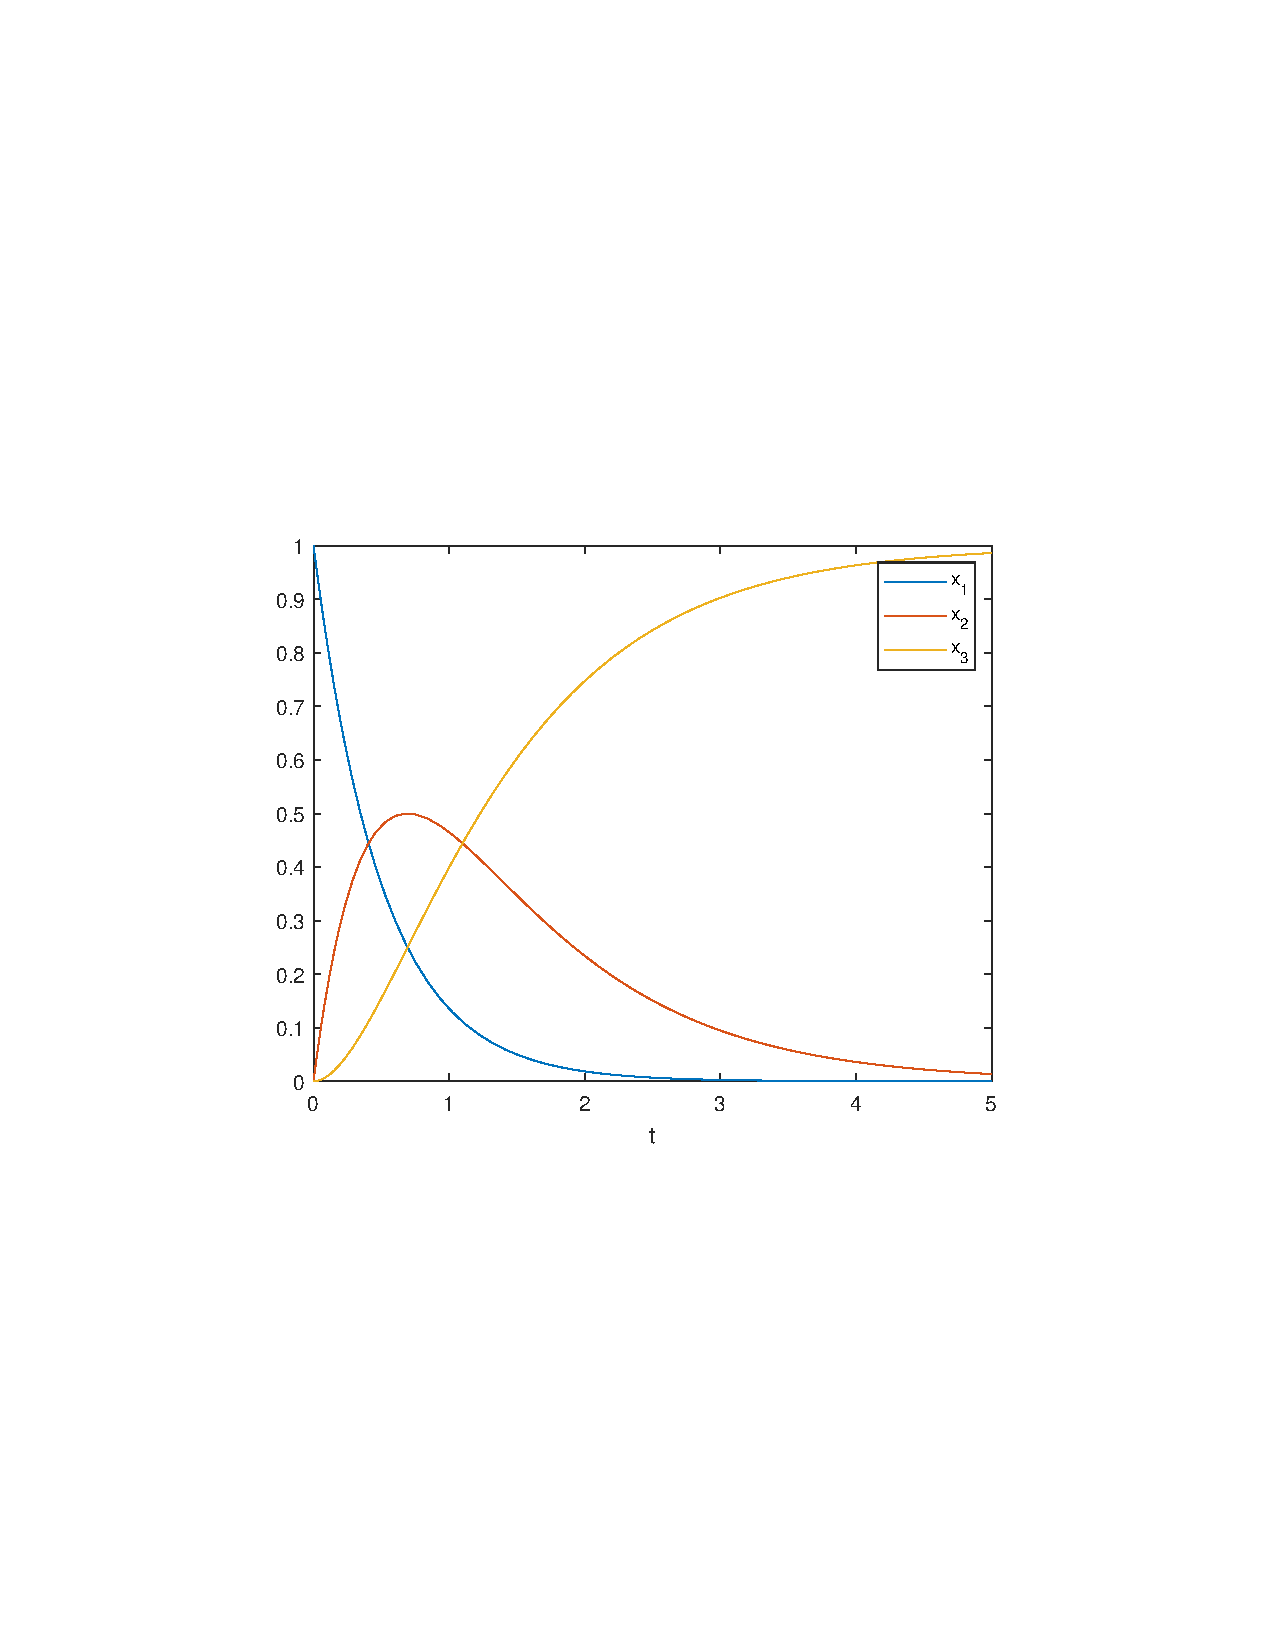
\includegraphics[width=\linewidth/2]{./code_ch1/exer1.pdf}
    \caption{system simulation}
    \label{fig:exer1-1}
\end{figure}
\end{answer}

\begin{exercise} Distributed systems and time delay.\\
We assume familiarity with the transfer function of a time delay from an undergraduate systems course
\begin{equation}
    \bar{y}(s)=e^{-\theta s}\bar{u}(s)
\end{equation}
Let's see the connection between the delay and the distributed systems, which give rise to it. A simple physical example of a time delay caused by transport in a flowing system. Consider plug flow in a tube depicted in Fig.\ref{fig:exer1-2}.

\begin{figure}[htbp]
\centering
\tikzset{every picture/.style={line width=0.75pt}} %set default line width to 0.75pt        
\begin{tikzpicture}[x=0.75pt,y=0.75pt,yscale=-1,xscale=1]
%uncomment if require: \path (0,185); %set diagram left start at 0, and has height of 185

%Shape: Ellipse [id:dp19295851654284357] 
\draw   (272,42) .. controls (283.05,42) and (292,57.67) .. (292,77) .. controls (292,96.33) and (283.05,112) .. (272,112) .. controls (260.95,112) and (252,96.33) .. (252,77) .. controls (252,57.67) and (260.95,42) .. (272,42) -- cycle ;
%Straight Lines [id:da7486939098222503] 
\draw    (272,42) -- (399.44,42) ;
%Straight Lines [id:da3129886311233703] 
\draw    (272,112) -- (399.44,112) ;
%Shape: Arc [id:dp1273018290846848] 
\draw  [draw opacity=0] (399.44,42) .. controls (399.44,42) and (399.44,42) .. (399.44,42) .. controls (399.44,42) and (399.44,42) .. (399.44,42) .. controls (410.49,42) and (419.44,57.67) .. (419.44,77) .. controls (419.44,96.33) and (410.49,112) .. (399.44,112) -- (399.44,77) -- cycle ; \draw   (399.44,42) .. controls (399.44,42) and (399.44,42) .. (399.44,42) .. controls (399.44,42) and (399.44,42) .. (399.44,42) .. controls (410.49,42) and (419.44,57.67) .. (419.44,77) .. controls (419.44,96.33) and (410.49,112) .. (399.44,112) ;  
%Straight Lines [id:da8609030882922339] 
\draw    (123,76.67) -- (237.44,77.32) ;
\draw [shift={(239.44,77.33)}, rotate = 180.33] [color={rgb, 255:red, 0; green, 0; blue, 0 }  ][line width=0.75]    (10.93,-3.29) .. controls (6.95,-1.4) and (3.31,-0.3) .. (0,0) .. controls (3.31,0.3) and (6.95,1.4) .. (10.93,3.29)   ;
%Straight Lines [id:da8626778179325296] 
\draw    (437.44,77.33) -- (536.11,77.33) ;
\draw [shift={(538.11,77.33)}, rotate = 180] [color={rgb, 255:red, 0; green, 0; blue, 0 }  ][line width=0.75]    (10.93,-3.29) .. controls (6.95,-1.4) and (3.31,-0.3) .. (0,0) .. controls (3.31,0.3) and (6.95,1.4) .. (10.93,3.29)   ;

% Text Node
\draw (124,41.4) node [anchor=north west][inner sep=0.75pt]    {$c_{j} \ ( 0,t) =u( t)$};
% Text Node
\draw (124,84.4) node [anchor=north west][inner sep=0.75pt]    {$v$};
% Text Node
\draw (252,118.4) node [anchor=north west][inner sep=0.75pt]    {$z=0$};
% Text Node
\draw (390,123.4) node [anchor=north west][inner sep=0.75pt]    {$z=L$};
% Text Node
\draw (439,41.4) node [anchor=north west][inner sep=0.75pt]    {$c_{j} \ ( 0,t) =y( t)$};
\end{tikzpicture}
\caption{Plug-flow reactor}
\label{fig:exer1-2}
\end{figure}

\begin{enumerate}[label=(\alph*)]
    \item Write down the equation of change for moles of component $j$ for an arbitrary volume element and show that
    \begin{equation}
        \pdv{c_j}{t}=-\nabla \cdot (c_j v_j)+R_j
    \end{equation}
    in which $c_j$ is the molar concentration of component $j$, $v_j$ is the velocity of component $j$, and $R_j$ is the production rate of component $j$ due to chemical reaction.

    Plug flow means the fluid velocity of all components os purely in the $z$ direction, and os independent of $r$ and $\theta$ and, we assume here, z
    \begin{equation}
        v_j=v\delta_z
    \end{equation}
    
    \item Assuming plug flow and neglecting chemical reaction in the tube, show that the equation of change reduces to 
    \begin{equation}\label{equ:exer1-2}
        \pdv{c_j}{t}=-v\pdv{c_j}{z}
    \end{equation}
    This equation is known as a hyperbolic, first-order partial differential equation.
    \begin{alignat}{3}
        &c_j(z,t)=u(t) &&0=z &&t\ge 0  \\
        &c_j(z,t)=c_{j0}(t) \quad &&0\le z\le L\quad &&t=0 
    \end{alignat}
    In other words, we are using the feed concentration as the manipulated variable, $u(t)$, and the tube starts out with some initial concentration profile of component $j$, $c_{j0}(z)$.
    
    \item Show that the solution to \eqref{equ:exer1-2} with these boundary conditions is 
    \begin{equation}
        c_j(z,t) = 
        \begin{cases}
            u(t-z/v) & \quad vt>z\\
            c_{j0}(z-vt) & \quad vt<z\\ 
        \end{cases}
    \end{equation}
    \item If the reactor start out empty of component $j$, show that the transfer function between the outlet concentration, $y=c_j(L,t)$, and the inlet concentration, $c_j(0,t)=u(t)$, is a time delay. What is the value of $\theta$?
\end{enumerate}
\end{exercise}

\begin{answer}
\begin{enumerate}[label=(\alph*)]
    \item let $f$ be the moles of one of the component, then from 3D Leibniz formula, we get 
    \begin{equation}
        \pdv{c_j}{t}=\dv{}{t}\int_{V}f(\vec x,t)~\mathrm{d}V = 
        \int_V \pdv{f}{t}~\mathrm{d}V - 
        \int_A f\vec v\cdot \vec n\mathrm~{d}V
    \end{equation}
    where $V$ is a small unit volume, $A$ is the responding surface, $v$ represent the velocity of the point on the surface, $n$ is the outward unit normal vector related to $u$.\\
    By using Gauss divergence theorem, we know that
    \begin{equation}
        \int_V \pdv{f}{t}~\mathrm{d}V -
        \int_A f\vec v\cdot \vec n~\mathrm{d}V =
        \int_V \pdv{f}{t} - \nabla \cdot f\vec v~\mathrm{d}V = 
        -\nabla\cdot(c_j v_j)+R_j
    \end{equation} 
    where the last equation comes from $v_j=v\delta_z$.

    \item Neglecting chemical reaction in the tube, we get $R_j=0$. Then we know that
    \begin{equation}
        \pdv{c_j}{t}=-\nabla\cdot(c_j v_j)=
        -\left(\pdv{}{x}\delta_x+\pdv{}{y}\delta_y+\pdv{}{z}\delta_z\right)\cdot v\delta_z=-v\pdv{c_j}{z}
    \end{equation}

    \item Assuming that $u(t-z/v)=c_{j0}(z-vt)$ when $vt<z$, we just need to prove the solution is $c_j(z,t)=u(t-z/v)$. The variables of original partial differential equation has already been separated, so we get $c_j(z,t)=u(t-z/v)$ easily from the method of characteristics.

    \item We know that $y=u(t-L/v)$, which is a time delay. The value of $\theta$ could be $L/v$.
\end{enumerate}
\end{answer}


\begin{exercise} Pendulum in the state space.\\
    Consider the pendulum suspended at the end of a rigid link depicted in Figure \ref{fig:exer1-3}. Let $r$ and $\theta$ denote the polar coordinates of the center of the pendulum, and let $p=r\delta_r$ be the position vector of the pendulum, in which $\delta_r$ and $\delta_\theta$ are the unit vectors in polar coordinates. We wish to determine a state space description of the system. We are able to apply a torque $T$ to the pendulum as our manipulated variable. The pendulum has mass $m$, the only other external force acting on the pendulum is gravity, and we neglect friction. The link provides force $-t\delta_r$ necessary to maintain the pendulum at distance $r=R$ from the axis of rotation, and we measure the force $t$.
    \begin{enumerate}[label=(\alph*)]
        \item Provide expressions for the four partial derivatives for changes in the unit vectors with $r$ and $\theta$
        \begin{equation}
            \pdv{\delta_r}{r}\quad
            \pdv{\delta_r}{\theta}\quad
            \pdv{\delta_\theta}{r}\quad
            \pdv{\delta_\theta}{\theta}
        \end{equation}
        \item Use the chain rule to find the velocity of the pendulum in terms of the time derivatives of $r$ and $\theta$. Do not simplify yet by assuming $r$ is constant. We want the general result.
        \item Differentiate again to show that the acceleration of the pendulum is
        \begin{equation}
            \ddot{p}=(\ddot{r}-r\dot{\theta}^2)\delta_r+(r\ddot{\theta}+2\dot r\dot \theta)\delta_\theta
        \end{equation}
        \item Use a momentum balance on the pendulum mass (you may assume it is a point mass) to determine both the force exerted by the link
        \begin{equation}
            t=mR\dot{\theta}^2+mg\cos \theta
        \end{equation}
        and an equation for the pendulum due to gravity and the applied torque 
        \begin{equation}
            mR\ddot \theta-T/R+mg\sin \theta=0
        \end{equation}
        \item Define a state vector and give a state space description of your system. What is the physical significance of your state. Assume you measure the force exerted by the link. 

        One answer is 
        \begin{align}
            \dv{x_1}{t}&=x_2\\
            \dv{x_2}{t}&=-(g/R)\sin x_1 + u\\
            y&=mRx_2^2+mg\cos x_1
        \end{align}
        in which $u=T/(mR)$
    \end{enumerate}

    \begin{figure}[htbp]
        \centering
        \tikzset{every picture/.style={line width=0.75pt}} %set default line width to 0.75pt        
        \begin{tikzpicture}[x=0.75pt,y=0.75pt,yscale=-1,xscale=1]
        %uncomment if require: \path (0,314); %set diagram left start at 0, and has height of 314

        %Shape: Circle [id:dp2950011826534309] 
        \draw   (292,68.56) .. controls (292,63.52) and (296.08,59.44) .. (301.11,59.44) .. controls (306.14,59.44) and (310.22,63.52) .. (310.22,68.56) .. controls (310.22,73.59) and (306.14,77.67) .. (301.11,77.67) .. controls (296.08,77.67) and (292,73.59) .. (292,68.56) -- cycle ;
        %Straight Lines [id:da090033932413494] 
        \draw    (301.11,68.56) -- (301.11,296.11) ;
        %Straight Lines [id:da4699536388586447] 
        \draw    (301.11,77.67) -- (401.11,177.67) ;
        %Straight Lines [id:da6389033949732379] 
        \draw    (310.22,68.56) -- (410.22,168.56) ;
        %Shape: Circle [id:dp07724480337773221] 
        \draw   (397.56,191.11) .. controls (397.56,177.3) and (408.75,166.11) .. (422.56,166.11) .. controls (436.36,166.11) and (447.56,177.3) .. (447.56,191.11) .. controls (447.56,204.92) and (436.36,216.11) .. (422.56,216.11) .. controls (408.75,216.11) and (397.56,204.92) .. (397.56,191.11) -- cycle ;
        %Straight Lines [id:da5473757293168724] 
        \draw    (422.56,216.11) -- (422.56,295.78) ;
        \draw [shift={(422.56,298.78)}, rotate = 270] [fill={rgb, 255:red, 0; green, 0; blue, 0 }  ][line width=0.08]  [draw opacity=0] (8.93,-4.29) -- (0,0) -- (8.93,4.29) -- cycle    ;
        %Shape: Arc [id:dp03303639601363284] 
        \draw  [draw opacity=0] (340.52,49.02) .. controls (349.47,67.04) and (345.1,89.49) .. (328.82,102.7) .. controls (309.96,118.01) and (282.27,115.12) .. (266.97,96.27) .. controls (263.64,92.16) and (261.17,87.64) .. (259.54,82.92) -- (301.11,68.56) -- cycle ; \draw   (340.52,49.02) .. controls (349.47,67.04) and (345.1,89.49) .. (328.82,102.7) .. controls (309.96,118.01) and (282.27,115.12) .. (266.97,96.27) .. controls (263.64,92.16) and (261.17,87.64) .. (259.54,82.92) ;  
        %Straight Lines [id:da5790277832441415] 
        \draw    (340.52,49.02) -- (338.83,45.2) ;
        \draw [shift={(337.62,42.45)}, rotate = 66.18] [fill={rgb, 255:red, 0; green, 0; blue, 0 }  ][line width=0.08]  [draw opacity=0] (8.93,-4.29) -- (0,0) -- (8.93,4.29) -- cycle    ;
        %Shape: Arc [id:dp13698095777819153] 
        \draw  [draw opacity=0] (369.14,146.35) .. controls (362.68,152) and (355.4,156.92) .. (347.37,160.94) .. controls (332.57,168.36) and (316.83,171.88) .. (301.33,171.9) -- (301.11,68.56) -- cycle ; \draw   (369.14,146.35) .. controls (362.68,152) and (355.4,156.92) .. (347.37,160.94) .. controls (332.57,168.36) and (316.83,171.88) .. (301.33,171.9) ;  
        %Straight Lines [id:da16810105436476697] 
        \draw    (363.08,151) -- (366.76,148.18) ;
        \draw [shift={(369.14,146.35)}, rotate = 142.52] [fill={rgb, 255:red, 0; green, 0; blue, 0 }  ][line width=0.08]  [draw opacity=0] (8.93,-4.29) -- (0,0) -- (8.93,4.29) -- cycle    ;

        % Text Node
        \draw (430.58,241.07) node [anchor=north west][inner sep=0.75pt]    {$g$};
        % Text Node
        \draw (454.92,181.07) node [anchor=north west][inner sep=0.75pt]    {$m$};
        % Text Node
        \draw (336.67,168.32) node [anchor=north west][inner sep=0.75pt]    {$\theta $};
        % Text Node
        \draw (399.25,133.82) node [anchor=north west][inner sep=0.75pt]    {$r$};
        % Text Node
        \draw (351.67,55.9) node [anchor=north west][inner sep=0.75pt]    {$T$};

        \end{tikzpicture}
        \caption{Pendulum with applied torque}
        \label{fig:exer1-3}
        \end{figure}
\end{exercise}

\begin{answer}
\begin{enumerate}[label=(\alph*)]
    \item we assume that $\delta_\theta$ is rotated from $\delta$ by anticlockwise.
    \begin{equation}
        \pdv{\delta_r}{r}=0 \quad
        \pdv{\delta_r}{\theta}=\delta_\theta \quad
        \pdv{\delta_\theta}{r}=0 \quad
        \pdv{\delta_\theta}{\theta}=-\delta_r
    \end{equation} 
    \item Since $p=r\delta_r$
    \begin{equation}
        \dot p=\dot r\delta_r+r\pdv{\delta_r}{t}
        =\dot r\delta_r+r\pdv{\delta_r}{\theta}\dot\theta
        =\dot r\delta_r+r\dot\theta\delta_\theta
    \end{equation}
    \item Differentiate again
    \begin{align}
        \ddot p&=\ddot r \delta_r+\dot r\dot\theta\delta_\theta+r\ddot\theta\delta_\theta+r\dot\theta\left(-\delta_r\dot\theta\right)+\dot r\dot\theta\delta_\theta\\
        &=\left(\ddot r-r\dot\theta^2\right)\delta_r+\left(r\ddot\theta+2\dot r\dot\theta\right)\delta_\theta
    \end{align}
    \item By the Newton's second law of motion, we get
    \begin{equation}
        F=-t\delta_r+T/R \delta_\theta+mg\sin\theta\delta_r+mg\cos\theta\delta_\theta=-mR\dot\theta^2\delta_r
    \end{equation}
    Simplify it by two direction
    \begin{align}
        &t=mR\dot\theta^2+mg\cos\theta\\
        &mR\ddot\theta-T/R+mg\sin\theta=0
    \end{align}
    \item State vector could be $x=[\theta,\dot \theta]^\top$, and the system
    \begin{align}
        \dot x&=\begin{bmatrix}
            \dot \theta\\
            \ddot \theta
        \end{bmatrix}=
        \begin{bmatrix}
            \dot \theta\\
            -g\sin\theta/R+T/\left(mR^2\right)
        \end{bmatrix}\\
        y&=\theta
    \end{align}
\end{enumerate}
\end{answer}

\begin{exercise} Time to Laplace domain.\\
Take the Laplace transform of the following set of differential equations and find the transfer function, $G(s)$, connecting $\bar u(s)$ and $\bar y(s)$, $\bar y=G\bar u$
\begin{align}\label{equ:exer1-4}
    \dv{x}{t}&=Ax+Bu\\
    y&=Cx+Du
\end{align}
For $x\in\mathbb R^n$, $y\in\mathbb R^p$, and $u\in\mathbb R^m$, what is the dimension of the $G$ matrix? What happens to the initial condition, $x(0)=x_0$? 
\end{exercise}

\begin{answer}
The Laplace transform of the differential equation is 
\begin{equation}
    sx=Ax+Bu
\end{equation}
and the transfer function
\begin{equation}
    G(s)=C(sI-A)^{-1}B\in\mathbb{R}^{p\times m}
\end{equation}
the initial condition does not appear in the Laplace transform, because the Laplace transform explains the dynamic from $u$ to $y$, and when we need to determine the accurate trajectory of the system, the initial condition is needed by inverse Laplace transform.
\end{answer}

\begin{exercise} Converting between continuous and discrete time models.\\
Given a prescribed $u(t)$, derive and check the solution to \eqref{equ:exer1-4}. Given a prescribed $u(k)$ sequence, what is the solution to the discrete time model
\begin{align}
    x(k+1)&=\tilde Ax(k)+\tilde Bu(k)\\
    y(k)&=\tilde Cx(k)+\tilde Du(k)
\end{align}
\begin{enumerate}[label=(\alph*)]
    \item Compute $\tilde A$, $\tilde B$, $\tilde C$, and $\tilde D$ so that the two solutions agree at the sample times for a zero-order hold input, i.e., $y(k)=y(t_k)$ for $u(t)=u(k), t\in (t_k,t_{k+1})$ in which $t_k=k\Delta$ for sample time $\Delta$.
    \item Is your result valid for $A$ singular? If not, how can you find $\tilde A$, $\tilde B$, $\tilde C$, and $\tilde D$ for this case?
\end{enumerate}
\end{exercise}

\begin{answer}
\begin{enumerate}[label=(\alph*)]
    \item the solution to \eqref{equ:exer1-4} is
    \begin{equation}
        x(\Delta)=e^{A\Delta}x_0+\int_0^\Delta e^{A(\Delta-\tau)}Bu(\tau)\dd x
    \end{equation}
    so the accurate discrete time model is
    \begin{equation}
        \tilde{A}=e^{A\Delta}\quad\tilde B=\int_0^\Delta e^{A(\Delta-\tau)}B\dd x
        \quad\tilde{C}=C\quad\tilde{D}=D
    \end{equation}
    \item Yes, this result can be calculate normally even if A is singular.
\end{enumerate}
\end{answer}

\begin{exercise}Continuous to discrete time conversion for nonlinear models\\
Consider the autonomous nonlinear differential equation model 
\begin{align}\label{equ:exer1-6}
    \dv{x}{t}&=f(x,u)\\
    x(0)&=x_0
\end{align} 
Given a zero-order hold on the input, let $s(t,u,x_0),0\le t\le\Delta$, be the solution to \eqref{equ:exer1-6} given initial condition $x_0$ at the time $t=0$, and constant input $u$ is applied for $t$ in the interval $0\le t\le\Delta$. Consider also the nonlinear discrete time model
\begin{equation}
    x(k+1)=F(x(k),u(k))
\end{equation}
\begin{enumerate}[label=(\alph*)]
    \item What is the relationship between $F$ and $s$ so that the solution of the discrete time model agrees at the sample times with the continuous time model with a zero-order hold?
    \item Assume $f$ is linear and apply this result to check the result of Exercise 1.5.
\end{enumerate}
\end{exercise}

\begin{answer}
\begin{enumerate}[label=(\alph*)]
    \item The relationship is 
    \begin{equation}
        F(x(k),u(k))=s(\Delta,u(k-1),x(k-1))
    \end{equation}
    \item It is obvious.
\end{enumerate}
\end{answer}

\begin{exercise}Commuting functions of a matrix.\\
Although matrix multiplication does not commute in general
\begin{equation}
    AB\neq BA
\end{equation}
multiplication of functions of the same matrix do commute. You may have used the following fact in Exercise 1.5
\begin{equation}\label{equ:exer1-7}
    A^{-1}\exp{At}=\exp{At}A^{-1}
\end{equation}
\begin{enumerate}[label=(\alph*)]
    \item Prove that \eqref{equ:exer1-7} is true assuming $A$ has distinct eigenvalues and can therefore be represented as 
    \begin{equation}
        A=Q\Lambda Q^{-1}\quad 
        \Lambda=\begin{bmatrix}
            \lambda_1 &0 &\cdots &0\\
            0 &\lambda_2 &\cdots &0\\
            \vdots &\vdots &\ddots &\vdots\\
            0 &0 &\cdots &\lambda_n\\
        \end{bmatrix}
    \end{equation}
    in which $\Lambda$ is a diagonal matrix containing the eigenvalues of $A$, and $Q$ is the matrix of eigenvectors such that
    \begin{equation}
        Aq_i=\lambda_iq_i, \quad i=1,\cdots,n
    \end{equation}
    in which $q_i$ is the $i$th column of the matrix $Q$.
    \item Prove the more general relationship
    \begin{equation}\label{equ:exer1-7-2}
        f(A)g(A)=g(A)f(A)
    \end{equation}
    in which $f$ and $g$ are any functions definable by Taylor series.
    \item Prove that \eqref{equ:exer1-7-2} is true without assuming the eigenvalues are distinct.\\
    Hint: use the Taylor series defining the functions and apply the Cayley-Hamilton theorem\cite{rawlings2017model}.
\end{enumerate}
\end{exercise}

\begin{answer}
By using Cayley-Hamilton theorem, we know the matrix functions definable by Taylor series can be written in the sum of finite power terms of matrix A\cite{CayleyHamiltonTheorem}. So all the question is answered obviously by matrix commutability of finite power terms.
\end{answer}

\begin{exercise}Finite difference formula and approximating the exponential.\\
Instead of computing the exact conversion of a continuous time to a discrete time system as in Exercise 1.5, assume instead one simply approximates the time derivative with a first-order finite difference formula
\begin{equation}
    \dv{x}{t}\approx\dfrac{x(t_{k-1})-x(t_k)}{\Delta}
\end{equation}
with  step size equal to the sample time, $\Delta$. For this approximation of the continuous time system, compute $\tilde A$ and $\tilde B$ so that the discrete time system agrees with the approximate continuous time system at the sample times. Comparing these answers to the exact solution, what approximation of $e^{A\Delta}$ results from the finite difference approximation? When is this a good approximation of $e^{A\Delta}$?
\end{exercise}

\begin{answer}
In this case, the system function can be written as 
\begin{equation}
    \dfrac{x(t_{k+1})-x(t_k)}{\Delta}=Ax(t_k)+Bu(t_k)
\end{equation} 
which could be written as
\begin{equation}
    x(t_{k+1})=(I+\Delta A)x(t_k)+\Delta Bu(t_k)
\end{equation}
So $\tilde A=I+\Delta A$, $\tilde B=\Delta B$, and $e^{A\Delta}\approx I+\Delta A$. When $\Delta$ is small, this is a good approximation.
\end{answer}

\begin{exercise}Mapping eigenvalues of continuous time systems to discrete time systems.\\
Consider the continuous time differential equation and discrete equation
\begin{align}
    \dv{x}{t}&=Ax\\
    x^+&=\tilde Ax
\end{align}
and the transformation
\begin{equation}
    \tilde A=e^{A\Delta}
\end{equation}
Consider the scalar $A$ case.
\begin{enumerate}[label=(\alph*)]
    \item What $A$ represents an integrator in continuous time? What is the corresponding $A$ value for the integrator for discrete time?
    \item What $A$ give purely oscillatory solutions? What are the corresponding $\tilde A$?
    \item For what $A$ is the solution of the ODE stable? Unstable? What are the corresponding $\tilde A$?
    \item Sketch and label these $A$ and $\tilde A$ regions in two complex-plane diagrams.
\end{enumerate}
\end{exercise}

\begin{answer}
\begin{enumerate}[label=(\alph*)]
    \item In continuous time, $A=0$, and the corresponding $\tilde A=I$.
    \item $A$ with all eigenvalues on the image axis give purely oscillatory solutions, and the corresponding $\tilde A$ has all its eigenvalues on the unit circle.
    \item $A$ with all eigenvalues on the left-half plane give the solution of the ODE stable (right-half plane give the solution of the ODE unstable), and the corresponding $\tilde A$ has its all eigenvalues in the unit circle (out of the unit circle).
    \item See Fig.\ref{fig:exer1-9}. The orange area denote the stable $A$, and the blue area denote the unstable $A$.
\end{enumerate}
\begin{figure}[htbp]
    \centering

    \tikzset{every picture/.style={line width=0.75pt}} %set default line width to 0.75pt        

    \begin{tikzpicture}[x=0.75pt,y=0.75pt,yscale=-1,xscale=1]
    %uncomment if require: \path (0,300); %set diagram left start at 0, and has height of 300
    
    %Shape: Rectangle [id:dp41972077044956557] 
    \draw  [color={rgb, 255:red, 0; green, 0; blue, 0 }  ,draw opacity=0 ][fill={rgb, 255:red, 74; green, 144; blue, 226 }  ,fill opacity=0.3 ] (137.72,95.2) -- (277.06,95.2) -- (277.06,236.53) -- (137.72,236.53) -- cycle ;
    %Shape: Circle [id:dp17807459140017246] 
    \draw  [color={rgb, 255:red, 0; green, 0; blue, 0 }  ,draw opacity=0 ][fill={rgb, 255:red, 255; green, 255; blue, 255 }  ,fill opacity=1 ] (164.67,165.86) .. controls (164.67,142.27) and (183.8,123.14) .. (207.39,123.14) .. controls (230.99,123.14) and (250.11,142.27) .. (250.11,165.86) .. controls (250.11,189.46) and (230.99,208.59) .. (207.39,208.59) .. controls (183.8,208.59) and (164.67,189.46) .. (164.67,165.86) -- cycle ;
    %Shape: Circle [id:dp3951835450590713] 
    \draw  [fill={rgb, 255:red, 245; green, 152; blue, 35 }  ,fill opacity=0.3 ] (164.67,165.86) .. controls (164.67,142.27) and (183.8,123.14) .. (207.39,123.14) .. controls (230.99,123.14) and (250.11,142.27) .. (250.11,165.86) .. controls (250.11,189.46) and (230.99,208.59) .. (207.39,208.59) .. controls (183.8,208.59) and (164.67,189.46) .. (164.67,165.86) -- cycle ;
    %Shape: Axis 2D [id:dp2649968087855814] 
    \draw  (115.28,165.86) -- (295.89,165.86)(207.39,77.94) -- (207.39,249.78) (288.89,160.86) -- (295.89,165.86) -- (288.89,170.86) (202.39,84.94) -- (207.39,77.94) -- (212.39,84.94)  ;
    %Shape: Rectangle [id:dp3122182305712575] 
    \draw  [color={rgb, 255:red, 0; green, 0; blue, 0 }  ,draw opacity=0 ][fill={rgb, 255:red, 74; green, 144; blue, 226 }  ,fill opacity=0.3 ] (442.72,95.2) -- (512.39,95.2) -- (512.39,236.53) -- (442.72,236.53) -- cycle ;
    %Shape: Axis 2D [id:dp6823514523283494] 
    \draw  (350.62,165.86) -- (531.22,165.86)(442.72,77.94) -- (442.72,249.78) (524.22,160.86) -- (531.22,165.86) -- (524.22,170.86) (437.72,84.94) -- (442.72,77.94) -- (447.72,84.94)  ;
    %Shape: Rectangle [id:dp9907477927724002] 
    \draw  [color={rgb, 255:red, 0; green, 0; blue, 0 }  ,draw opacity=0 ][fill={rgb, 255:red, 245; green, 152; blue, 35 }  ,fill opacity=0.25 ] (373.06,95.2) -- (442.72,95.2) -- (442.72,236.53) -- (373.06,236.53) -- cycle ;
    
    % Text Node
    \draw (285.33,175.33) node [anchor=north west][inner sep=0.75pt]   [align=left] {Real};
    % Text Node
    \draw (218,74) node [anchor=north west][inner sep=0.75pt]   [align=left] {Image};
    % Text Node
    \draw (190.67,167.07) node [anchor=north west][inner sep=0.75pt]    {$O$};
    % Text Node
    \draw (252.11,169.26) node [anchor=north west][inner sep=0.75pt]    {$1$};
    % Text Node
    \draw (520.67,175.33) node [anchor=north west][inner sep=0.75pt]   [align=left] {Real};
    % Text Node
    \draw (453.33,74) node [anchor=north west][inner sep=0.75pt]   [align=left] {Image};
    % Text Node
    \draw (426,167.07) node [anchor=north west][inner sep=0.75pt]    {$O$};
    
    
    \end{tikzpicture}
    
    \caption{Stable and Unstable $A$ and $\tilde A$ in two complex plane}
    \label{fig:exer1-9}
    \end{figure}
\end{answer}

\begin{exercise}State space realization\\
Define a state vector and realize the following models as the state models by hand. One should do a few by hand to understand what the Octave or MATLAB calls are doing. Answer the following questions. What is the connection betweenthe poles of $G$ and the state space description? For what kinds of $G(s)$ does one obtain a nonzero $D$ matrix? What is the order and gain of these systems? Is there a connection between order and the numbers of inputs and outputs?
\begin{enumerate}[label=(\alph*)]
    \item $$G(s)=\dfrac{1}{2s+1}$$
    \item $$G(s)=\dfrac{1}{(2s+1)(3s+1)}$$
    \item $$G(s)=\dfrac{2s+1}{3s+1}$$
    \item $$y(k+1)=y(k)+2u(k)$$
    \item $$y(k+1)=a_1 y(k)+a_2 y(k-1)+b_1 u(k)+b_2 u(k-1)$$
\end{enumerate}
\end{exercise}

\begin{answer}
\begin{enumerate}
    \item 
\end{enumerate}
\end{answer}


































% \chapter{Appendix A. Mathematical Background}
% Since the mathematical background is basic, we jump to the exercises section.
% \section{The solution of Exercises}
% \begin{exercise} Norms in $\mathbb{R}^n$\\
% Show that the following three functions are all norms in $\mathbb{R}^n$

% \begin{equation}\notag
%     \|x\|_2 
% \end{equation}

% \end{exercise}

\bibliographystyle{unsrt}
\bibliography{mybib}

\end{document}






















